\chapter{Produktudvikling}\label{Produktudvikling} 

\section{Systemarkitektur}\label{Systemarkitektur}
Der er udarbejdet forskellige arkitektur-diagrammer på baggrund af de specificerede systemkrav. Diagrammerne har til formål at beskrive Automatisk Ultralydsscanner som et overordnet system.

Arkitekturen beskriver den grundlæggende organisering af Automatisk Ultralydsscanner og opbygningen af dens tilhørende PC Applikation. Der er i diagrammerne designet ud fra, at 3D kamera er af typen Microsoft Kinect 2.0 og Robotarm er en Universal Robot UR10 robot. For detaljeret gennemgang af systemarkitektur for Automatisk Ultralydsscanner se Bilag  \ref{Udviklingsdokument} Udviklingsdokument
\subsection{Domænemodel}
Nedenstående diagram på Figur \ref{domain} viser de overordnede moduler og tydeliggør forbindelserne samt interaktionerne mellem de forskellige aktører i Automatisk Ultralydsscanner. 

\begin{figure}[H]
    \centering
    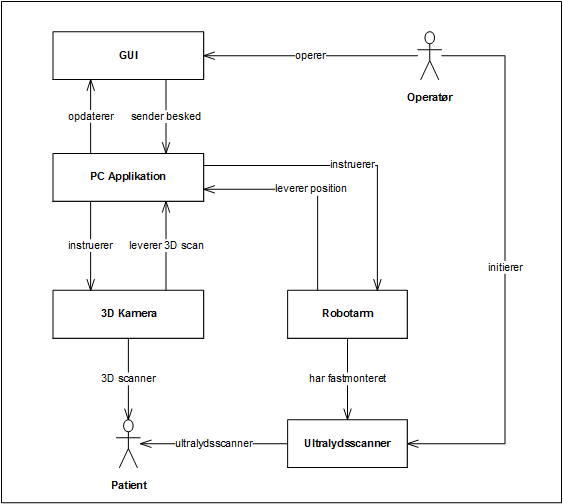
\includegraphics[width=0.6\textwidth]{figurer/d/Design/uml_domain}
    \caption{Domænemodel for Automatisk Ultralydsscanner}
    \label{domain}
\end{figure}

\subsection{Block definition diagram}
Automatisk Ultralydsscanner består af Robotarm, en computer, et Access Point, 3D kamera og Ultralydsscanner. Det er vigtigt at bemærke, at computer skal have PC Applikationen installeret og en mus og en skærm for at Operatør kan intergere med PC Applikation. Block Definitions diagrammet viser Figur \ref{BDD}, hvordan systemets blokke er forbundet. 

\begin{figure}[H]
    \centering
    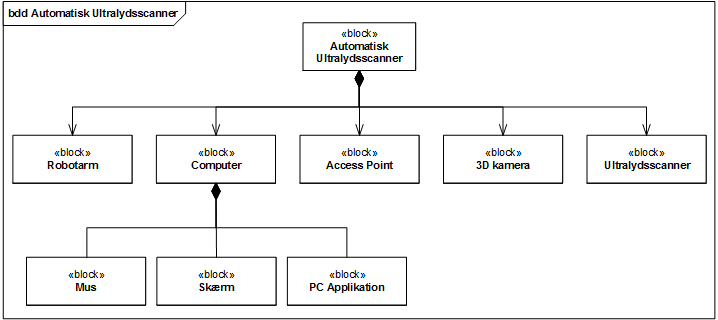
\includegraphics[width=1\textwidth]{figurer/d/Design/BDD}
    \caption{BDD for Automatisk Ultralydsscanner}
    \label{BDD}
\end{figure}

\subsection{Internal block diagram}
Detaljerne mellem interaktionen mellem de enkelte blokke er beskrevet i internal block diagram Figur \ref{IBD}, som viser systemets interne forbindelser og flow mellem de forskellige blokke. Bemærk at Ultralydsscanner ikke er inkluderet her, da den ikke har forbindelse til de andre blokke udover at være monteret mekanisk på Robotarm. Forbindelsen mellem PC Applikation og Access Point, samt Acces Point og Robotarm er oprettet med ethernet-kabler. 3D kamera forbindes til PC Applikation gennem USB.

\begin{figure}[H]
    \centering
    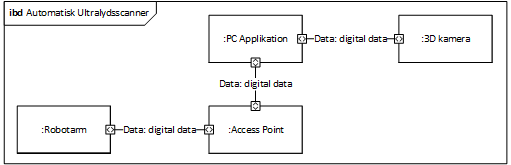
\includegraphics[width=0.8\textwidth]{figurer/d/Design/IBD}
    \caption{IBD for Automatisk Ultralydsscanner}
    \label{IBD}
\end{figure}

\section{Systemdesign} \label{Systemdesign}
Systemdesignet beskriver hvordan PC Applikation er opbygget og hvordan PC Apllikations klasser integrerer med hinanden.  

Nedenfor vil relevante diagrammer blive gennemgået. For detaljeret gennemgang af systemdesign for Automatisk Ultralydsscanner se Bilag  \ref{Udviklingsdokument} Udviklingsdokument.

\subsubsection{Klassediagram}
Klassediagrammerne viser strukturen i PC Applikations klasser og afhængihederne mellem disse. Hver klasse i diagrammerne indeholder de vigtigste metoder og attributer fra klassen, der udgør funktionaliteten i PC Applikation. 

For et overblik over funktionaliteten i PC Applikation kan der tages udgangspunkt i klassediagrammet for den grafiske brugergrænseflade på figur \ref{class_gui}.

\begin{figure}[H]
    \centering
    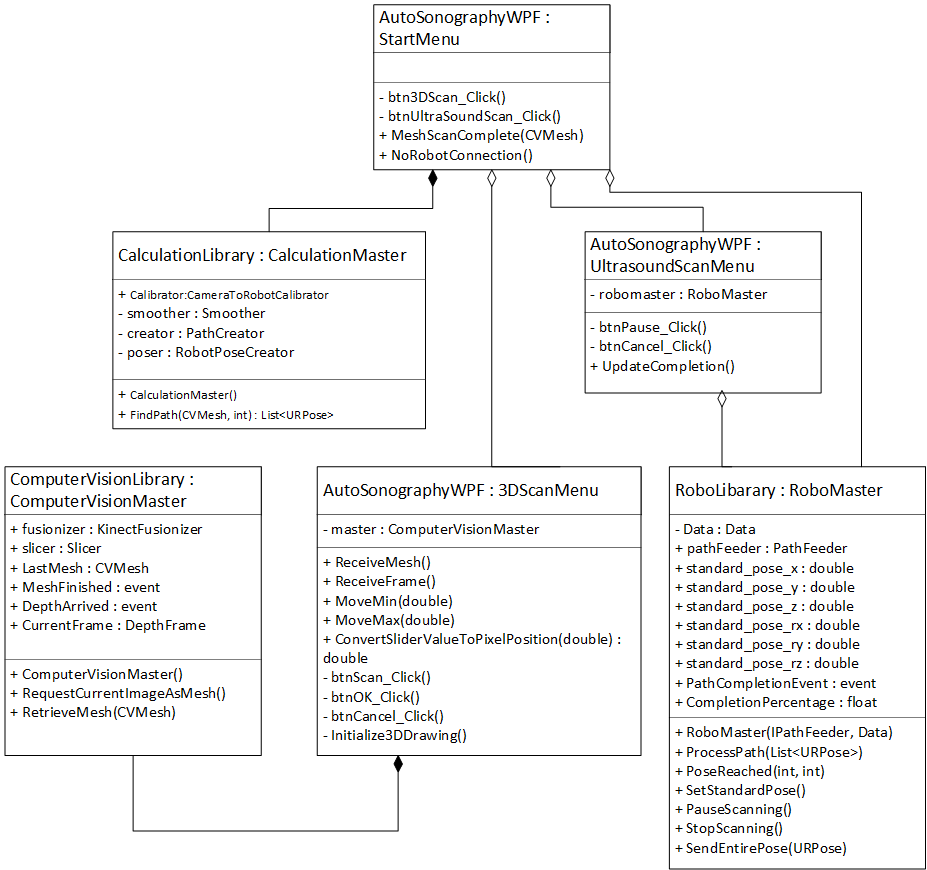
\includegraphics[width=1\textwidth]{figurer/d/Design/Class/uml_class_gui}
    \caption{Klassediagram for GUI}
    \label{class_gui}
\end{figure}

\newpage

\let\labelitemi\labelitemii
\begin{itemize}
\item{MainWindow}\newline
Giver anledning til at foretage et 3D scan. Såfremt en 3D scanning er gennemført giver det også anledning til at starte en ultralydsscanning.
Når denne menu startes, oprettes en instans af RoboMaster, for at sætte Robotarm i standard positur. Dette er nødvendigt, hvis Robotarm skulle være i vejen for en 3D scanning.
Hvis der ikke er nogen forbindelse til Robotarm vil der vises en prompt med en besked om dette.

\item{3DScanMenu}\newline
I denne menu er der mulighed for at se det nuværende dybdebillede, afgrænse området der skal 3D scannes og foretage en 3D scanning.

\item{UltrasoundScanMenu}\newline
I denne menu kan den procentvise færdiggørelse af ultralydsscanningen følges. Der er også mulighed for at pause samt afbryde ultralydsscanningsprocessen.
\end{itemize}

For at få en dybere forståelse af logik og data-kommunikationen i ComputerVisionLibrary, CalculationLibrary samt RoboLibrary, se klassediagrammerne for de enkelte biblioteker i !!HUSK REFERENCE HER

\section{Udviklingsmiljø} 
Som integreret udviklingsmiljø er der blevet brugt Visual Studio. Dette er blevet valgt fordi  et tidligere bachelorprojekt med samme Robotarm har kodet i C\#, og fordi KinectAPI'et der anvendes understøtter C++ samt C\#.


